\chapter{Two-sided matching model on Japanese FDI}
\label{chap:FDI}

In the 1980s and 1990s, Japan FDI began to surge, becoming the second largest
source of FDI flow behind only the United States. An important factor behind
this development is the to float the hitherto undervalued yen. As the yen began
to rise in the 1980s and peak in 1995 against the dollar,
Japanese companies invested heavily abroad as they could now buy foreign assets
for cheap \citet{Delios2001}.

During this period, Japanese FDI also shifted its focus away from the US and
Europe, making Asia its top destination. Some scholars
have argued that this wave of Japanese FDI was instrumental to Asia's
economic growth by bringing not just capital but also technological know-how and
the opportunity to become integrated in the global production network. In this
so-called ``flying geese'' model of economic development, industrial development
spread from Japan, the leading goose, to the rest of Asia, e.g. the Four Asian
Tigers (Hong Kong, Singapore, South Korea, Taiwan), ASEAN, China, etc.
\citep{Bernard1995, Kojima2000}.

In this section, I apply the two-sided matching model to analyze the
location pattern of manufacturing Japanese MNCs in Asia, estimating the MNCs'
and countries' preference for each other.

\section{Data and sample choice}

The dataset was compiled by Andrew Delios from the \textit{Kaigai Shinshutsu
  Kigyou Souran} (Japanese Overseas Investments-by Country), 1986-1999 editions,
a biennial publication that contains operational data on all foreign affiliates
of Japanese firms.\footnote{I thank Professor Andrew Delios for generously
  sharing the data.} Tokyo Keizai, Inc. collects this data via a survey of these
affiliates, which is reputed to include all Japanese firms overseas
\citep{Yamawaki1991}. Comparing the Japanese Overseas Investment data with other
data sources on publicly listed firms, \citep{Delios2001} finds that the dataset
covers 98.5\% of public firms, which in turn control 99.5\% of the foreign
subsidiaries. This high level of coverage ensures that our data captures the
entire set of options available to countries and firms, obviating any worry
about whether the choice set in the data represents the choice set in
reality.\footnote{The mismatch between the choice set in the sample and in the
  population is an unexplored theoretical aspect of two-sided matching models.
  Consider an example where we analyze a sample of 1000 men and women in the US
  to estimate their mate preferences. How are our estimates affected by our
  assumption that the potential choice set of each man includes all the women
  (and vice versa)? Not only does an individual not have that many
  acquaintances, his social circle is also not a representative sample of the
  entire dataset \citep[568]{Logan2008}. Fortunately, this is not a problem for
  our application. Given that there are only 9 Asian investment locations and
  approximately 200 Japanese subsidiaries being built each year, we can
  reasonably assume that they are all available to one another as potential
  options.}

From this dataset, I make several choices restricting the sample to better fit
with the assumption of the two-sided matching model.

First, I limit the sample to manufacturing subsidiaries in Asia so that it is reasonable
for our model to assume
that all subsidiaries have the same set of preference parameters. Indeed,
\citep{Pak2005} finds that Japanese FDI in the West and in the East are
fundamentally different---While subsidiaries in the West seek
to augment their asset via R\&D and marketing, the subsidiaries in the East seek to exploit their
asset by setting up local production with Japanese management. In addition, manufacturing FDI mainly
consists of capital in the forms of property, plant, and equipment.
Therefore, our data on the size of their capital maps more precisely to the
concept of illiquid capital subjecting to the ``obsolescing bargain'' in
Political Science theories.

Second, I limit the sample to subsidiaries that are founded in the year 1996. The
reason to limit the sample to subsidiaries founded in a particular year instead
of including subsidiaries that have already invested is because the MNCs'
utility function in our model does not capture the fixed cost of relocating.
Indeed, as a linear combination of only country covariates, the utility function
does not take into account the fact that, if the moving cost is too high, a
subsidiary may not relocate to a new country even if the new country is
available and is a better option. Therefore, the utility function in our model
is not appropriate for subsidiaries that have already invested.\footnote{Past
applications of the two-sided matching model ignore this point and do not limit
their sample to only agents that are participating in the matching market around
the same time \citep{Logan1996, Logan2008}. However, given that a defining
characteristic of FDI is its relative immobility compared to other form of
global capital, the model's assumption of zero switching cost would be too
unreasonable if we do not limit our sample.}

While the decision to limit the sample to subsidiaries founded in a particular
year is theoretically motivated, the decision to choose the particular year of
1996 is simply to get the largest sample size. There may be concerns about 1996
being unique as a boom time leading up to the 1997 Asian Financial Crisis.
However, our sample only includes manufacturing FDI, which, unlike equity
investors and land developers, were largely unaffected by the financial crisis.
In addition, FDI trend remains stable before and after the crisis in terms of
inflow, exit rate, and profitability \citep{Delios2001, UNCTAD1998}. In
hindsight, this is not surprising as FDI firms focus on countries' fundamentals
and were thus unaffected by the fluctuations in the financial markets
\citep{Ahlquist2006}.

The final sample includes 6474 Japanese foreign affiliates in 2003, spreading
across 37 countries, with China being a top conte
for Japanese MNCs (Table \ref{tab:list_of_countries}).

\section{Variables}

For subsidiaries' characteristics that countries consider, I include:

\begin{itemize}
\item Capital size (in real US\$): A main argument for the benefit of FDI is
  that it brings capital to the country, improving labor productivity. MNCs'
  capital is especially important for developing countries, which often cannot
  muster much domestic capital from their poor population and underdeveloped
  financial market.

\item Labor size (number of employees): Similarly, a reputed benefit of FDI is
  that it creates jobs, generating not just economic growth but also increasing
  the government's popularity among the populace.

\item R\&D intensity (amount spent in R\&D as a percentage of revenue): To
  measure a subsidiary's technological capability, I use the R\&D intensity of
  the parent firm, calculated as the amount spent on R\&D as a percentage of
  revenue. Using the parent firm's R\&D intensity is a reasonable proxy because
  Japanese FDI in Asia is mainly asset exploitation, i.e. implementing the
  know-how developed at the parent firm to the production at the subsidiary
  \citep{Pak2005}.\footnote{Another measurement of a firm's intangible asset
    frequently used in the FDI literature is marketing intensity
    \citep{Girma2005}. Here I focus on R\&D intensity because it is the more
    important factor for manufacturing firms.}

\item Export intensity (amount earned via export as a percentage of revenue):
  Scholars have argued that economic growth in Asia is fueled by export and FDI
  as two mutually reinforcing forces \citep{Liu2002}. The subsidiary of an
  export-focused parent firm may help local suppliers become integrated into
  the global production network, improving the quality of their goods to match
  global standards and eventually being able to export themselves. Therefore, it
  would be interesting to test if countries actively look for investment from
  Japanese firms with an export focus.
\end{itemize}

For countries' characteristics that MNCs consider, I include the following
variables from the Penn World Table:

\begin{itemize}
\item Market size (log GDP, constant 2005 USD): MNCs are expected to prefer countries with a large market
  size, which present MNCs with many potential customers and suppliers. In
  addition, market size is a key variable in the gravity
  model, a standard model for analyzing FDI flows \citet{Bergstrand2007}.

\item Level of development (log GDP per capita, constant 2005 USD): As a measure
  of country income, development should attract more MNCs as MNCs prefer
  countries  with
  more disposable income to consume. On the other hand, as a measure of
  countries' capital
  abundance, development should reduce FDI inflow as MNCs' capital is no longer
  a big advantage.

\item Human capital (Penn World Table index): As one primary factor of
  production, labor matters greatly to firms' productivity and profit. To
  measure labor quality, the human capital index developed for the Penn World
  Table, which includes not only years of education but also labor productivity
  \citep{Feenstra2015}. Because the human capital index does not have a
  substantively interpretable unit, I standardize the variable so that it has a
  standard deviation of 1.
\end{itemize}

In sum, the model for the utility functions are:

\begin{itemize}
\item MNC $i$ utility for country $j$: $U_i(j) = \bm{\alpha}' W_j $, where $W_j$ includes log GDP, log GDP per capita, and human capital index.
\item Country $j$ utility for MNC $i$: $V_j(i) = \beta_{0j} + \bm{\beta_j}'
  X_i$, where $X_i$ includes log number of employees, log capital size, R\&D intensity, and
export intensity. 
\end{itemize}

\section{Result}
\label{sec:result}

The results below are produced by an MCMC chain with $4e6$ iterations with a
thinning interval of 10, resulting in $4e5$ saved iterations. The starting
values for all preference parameters are set at 0. I put a diffuse prior on
$\alpha$, specifically a Normal distribution with mean 0 and variance 100.

As discussed in Section~\ref{sec:reservation_choice}, since our sample does not include MNCs that choose the reservation choice, i.e. staying home instead of
investing abroad, the estimate for the $\beta$ intercept will be too high. To
combat this problem, I use an informative prior so that $\beta_{0j}$
approximately follows a Normal distribution with mean -1 and variance
10.\footnote{Specifically, the prior for $\beta_{0j}$'s mean is Normal with mean
  -1 and variance 1. The prior for $\beta_{0j}$'s variance is
  Inverse-Wishart with $\nu = 7$ and $S^{-1} = 10$ so that the variance is
  loosely centered around 10.}

Figure~\ref{fig:japan96_alpha} shows the posterior distribution and the 95\%
credible interval for MNCs' preference parameters. We can interpret the
parameters as the relative weight MNCs attach to countries' characteristics when
they decide where to invest. For example, the posterior mean for log GDP and for
log GDP per capita is 0.72 and 0.66---this means that to MNCs, a 1\% increase
in GDP is equivalent to 0.72 / 0.66 = 1.09\% increase in log GDP per capita.

The coefficients for log GDP and log GDP per capita are both positive and
significant, suggesting that Japanese MNCs are looking for large markets with a
lot of disposable income. On the other hand, the coefficient for human capital
is negative, corroborating earlier findings in the literature that Japanese MNCs
in Asia do not aim to be innovative and thus have no need for strong human
capital. On the contrary, since the human capital index includes not only years of
education but also labor productivity, a high human capital index may signify
high labor cost, explaining why Japanese manufacturing MNEs weigh it negatively. 

\begin{figure}[tbp] \centering
  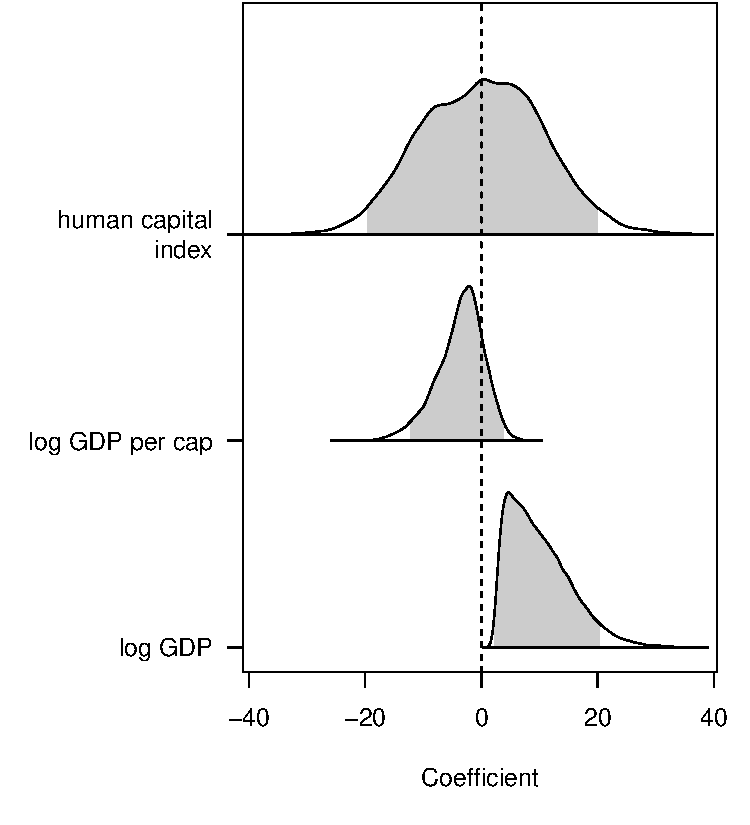
\includegraphics[width=0.75\textwidth,keepaspectratio]{japan96_alpha}
  \caption{Preference of MNCs for countries' characteristics. The density plot
    and the shaded region show the posterior distribution and the 95\% credible
    interval.}
  \label{fig:japan96_alpha}
\end{figure}

In addition to interpreting the coefficients as weights in the MNCs' utility
function, we can also simulate and visualize their impact on MNCs' location
choice. For example, we may ask if country A's GDP increases by 20\%, what will
be the new share of MNCs that invest in country A? Like in the one-sided
conditional logit model, the share of MNCs investing in a country depends not
only on country A's characteristics but also on others'. In addition, in this
two-sided model, the share of MNCs investing in a country also depends on the
preference of countries. For example, even if country A becomes highly
desirable, we may not see much change in the share of MNCs located there if
country A's preference is also highly demanding. The interaction can be much
more complicated. For example, consider a scenario in which country A and
country B have similar preferences and compete for the same set of MNCs---even
if country A becomes more desirable than the rest of the countries, as long as
country A is less attractive than country B, the share of MNCs investing in
country A will still remain unchanged.

Fortunately, we can easily simulate these effects in the Bayesian framework. To
see how the share of MNCs investing in Thailand changes along with hypothetical
values of Thailand's GDP, we can take the following steps:

\begin{enumerate}
  \item Construct a scenario in which Thailand has a new GDP, while all other
    characteristics remain for Thailand and other countries
  \item Make one draw for each parameter in the model from its posterior
    distribution
  \item Simulate the matching process in which countries first make offers to
    MNCs, and MNCs then choose the best option
  \item Record the share of MNCs investing in Thailand after the matching process
  \item Repeat step (2)-(4) to get a distribution for the share of MNCs in
    Thailand\footnote{Essentially we are constructing the posterior predictive
      distribution for the share of MNCs in Thailand, integrating out the
      preference parameters via simulation.}
\end{enumerate}

Following this process, I calculate the share of Japanese MNCs in Thailand at
different hypothetical values of Thailand's GDP.
Figure~\ref{fig:japan96_effect_GDP_on_share_of_MNCs} shows that as Thailand's
GDP changes between 50\% to 150\% of its true value, the share of MNCs in
Thailand changes between 8\% to 15\%. In addition, 

\begin{figure}[!ht]
  \centering
  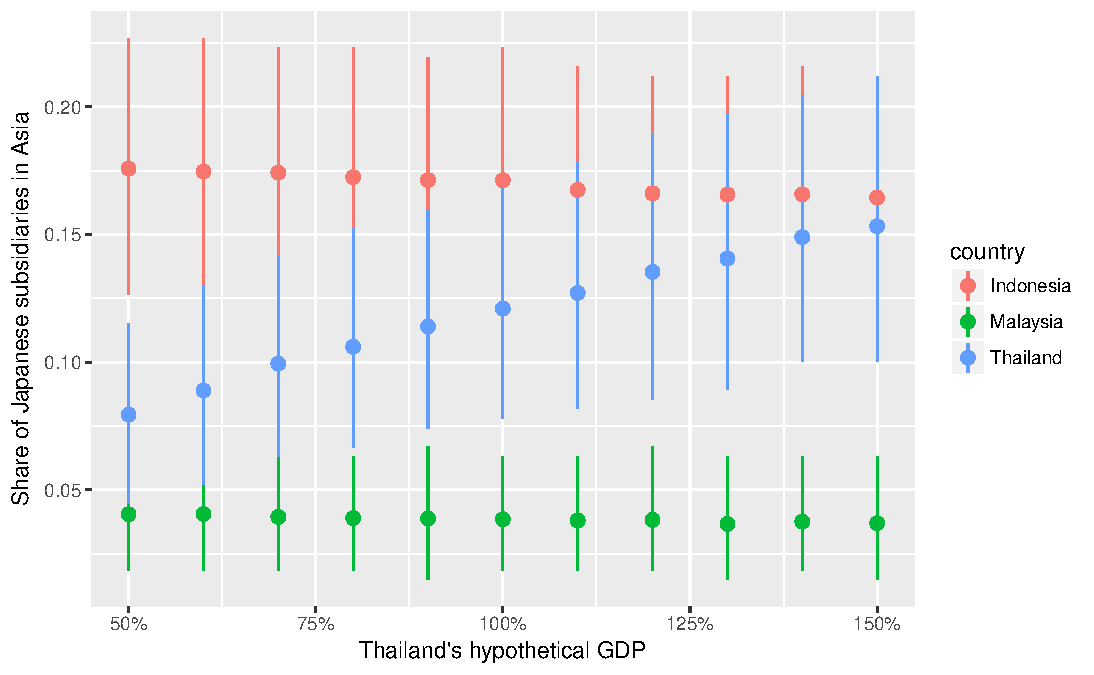
\includegraphics[width=\textwidth,keepaspectratio]{../figure/japan96_effect_GDP_on_share_of_MNCs}
  \caption{Thailand hypothetical GDP}
  \label{fig:japan96_effect_GDP_on_share_of_MNCs}
\end{figure}

\begin{figure}[tbp] \centering
  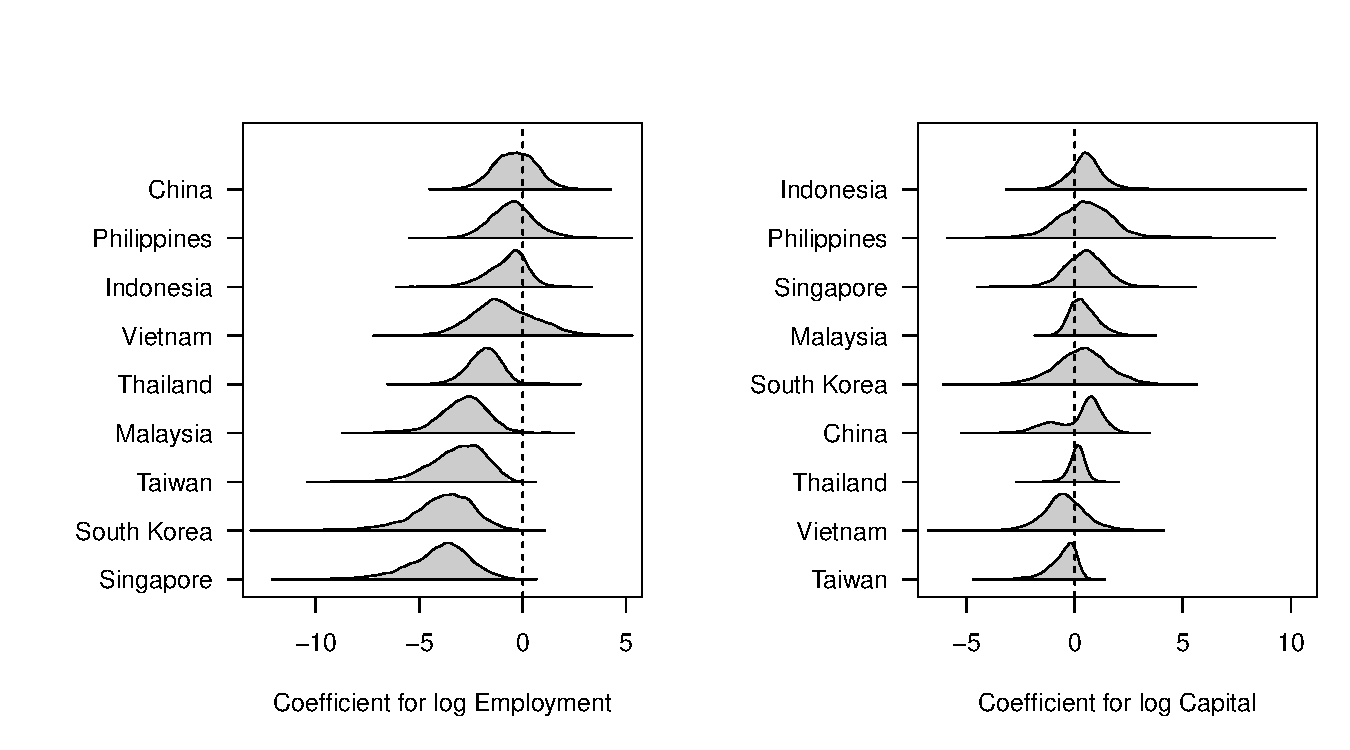
\includegraphics[width=\textwidth,keepaspectratio]{japan96_beta_ltemp_luscptl}
  \caption{Preference of countries for firms' size, measured by their labor
    force (left) and capital (right). The density plot and the shaded region
    show the posterior distribution and the 95\% credible interval.}
  \label{fig:japan96_beta_ltemp_luscptl}
\end{figure}

\begin{figure}[!ht] \centering
  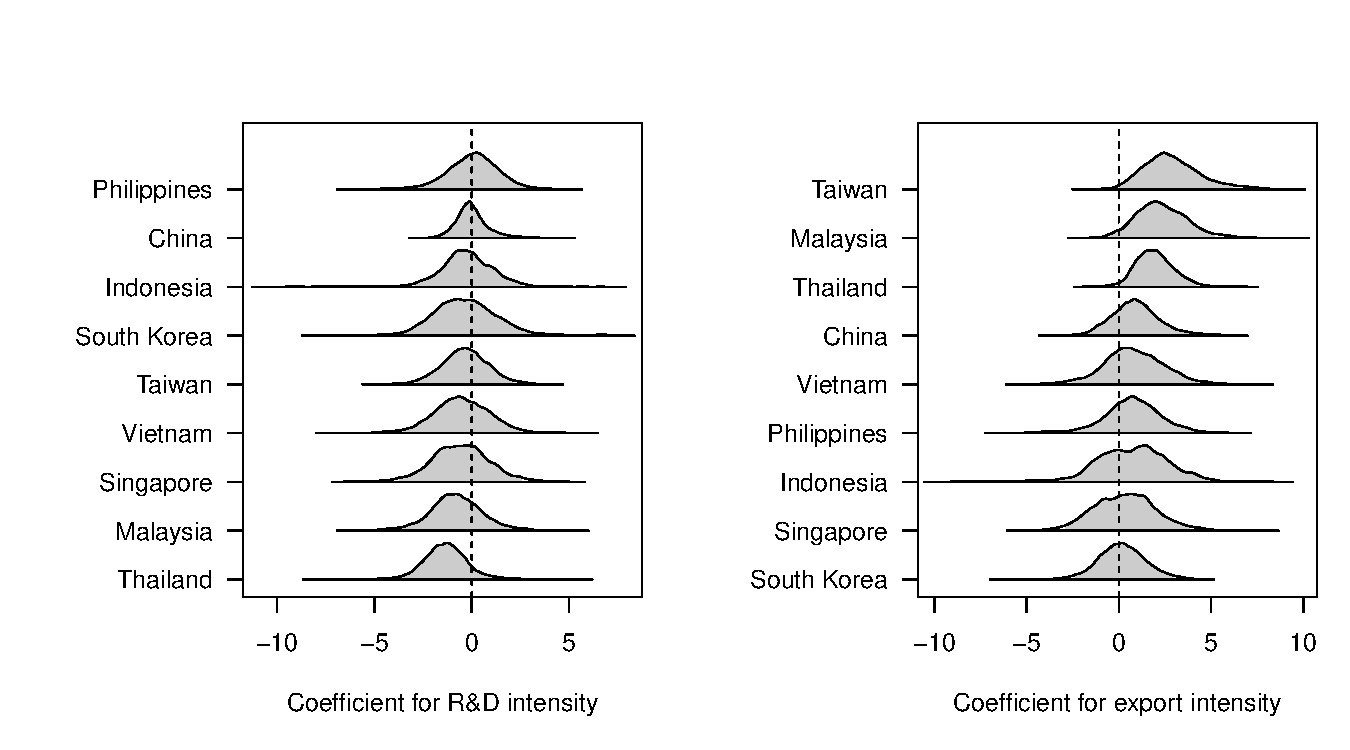
\includegraphics[width=\textwidth,keepaspectratio]{japan96_beta_intrd_intexp}
  \caption{Preference of countries for firms' intangible assets, i.e R\&D
    intensity (left) and export intensity (right). The density plot and the
    shaded region show the posterior distribution and the 95\% credible
    interval.}
  \label{fig:japan96_beta_intrd_intexp}
\end{figure}

\begin{figure}[!ht]
  \centering
  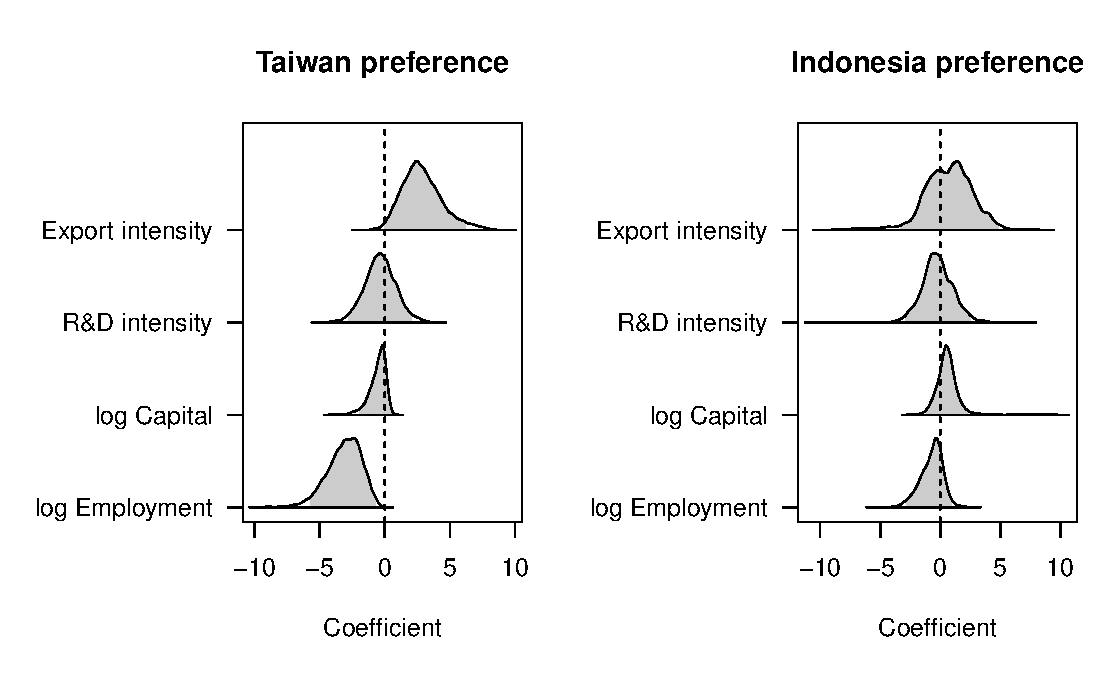
\includegraphics[width=\textwidth,keepaspectratio]{../figure/japan96_beta_Taiwan_Indonesia}
  \caption{Preference of Taiwan and Indonesia}
  \label{fig:japan96_beta_Taiwan_Indonesia}
\end{figure}



\begin{figure}[!ht]
  \centering
  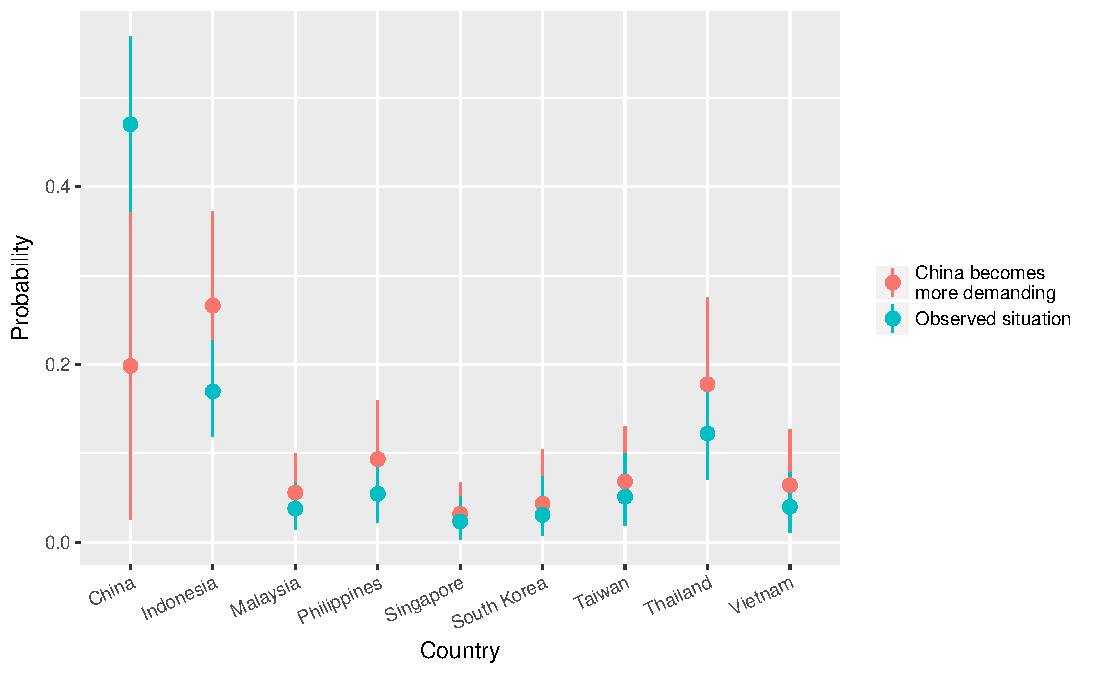
\includegraphics[width=\textwidth,keepaspectratio]{../figure/japan96_sim_china_more_demanding}
  \caption{China more demanding}
  \label{fig:japan96_sim_china_more_demanding}
\end{figure}

\section{Model fit}
\label{sec:model_fit}

\begin{figure}[!ht] \centering
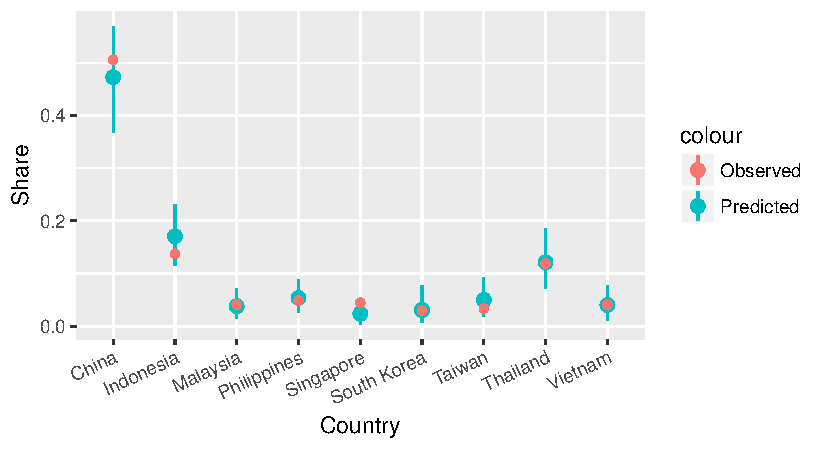
\includegraphics[width=\textwidth,keepaspectratio]{japan96_prob_being_chosen_by_MNC_two_sided}
  \caption{Predicted and observed probabilities that an MNC chooses to locate in
a country, conditional on the preference of countries. The point and the error
bar show the posterior mean and the 95\% credible interval.}
  \label{fig:japan96_prob_being_chosen_by_MNC_two_sided}
\end{figure}

Profiles of firms

\begin{figure}[!ht] \centering
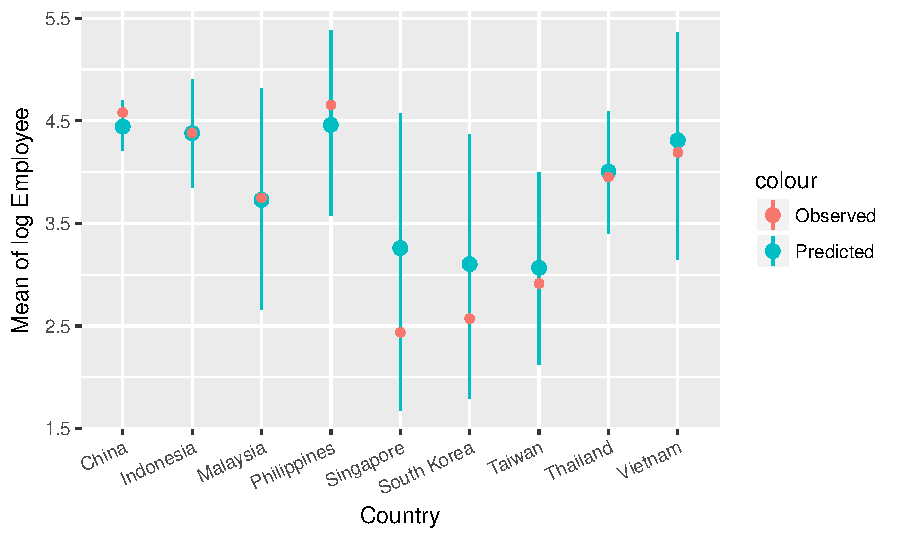
\includegraphics[width=\textwidth,keepaspectratio]{japan96_sim_mean_ltemp}
  \caption{Average of MNCs' labor size across countries. The point and the error
bar show the posterior mean and the 95\% credible interval.}
  \label{fig:japan96_sim_mean_ltemp}
\end{figure}

\begin{figure}[!ht] \centering
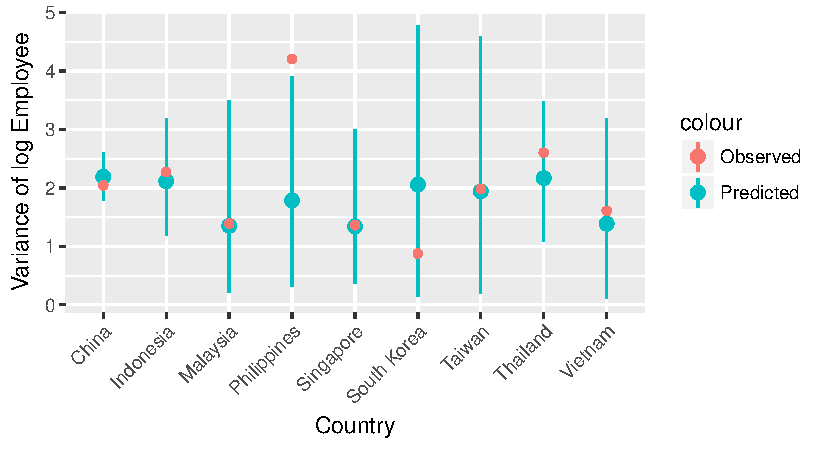
\includegraphics[width=\textwidth,keepaspectratio]{japan96_sim_var_ltemp}
  \caption{Variance of MNCs' labor size across countries. The point and the
error bar show the posterior mean and the 95\% credible interval.}
  \label{fig:japan96_sim_var_ltemp}
\end{figure}

%%% Local Variables:
%%% mode: latex
%%% TeX-master: "AnhLe_dissertation.tex"
%%% End: